\section{Results}\label{sec:result}
The measured $\sigma_{\mathrm{ABS}}$ and $\sigma_{\mathrm{CX}}$ are presented in Table \ref{tbl:result} and shown in Fig. \ref{fig:result} with statistical and systematic error bars as a function of pion momentum, compared with the results from previous experiments \cite{Bellotti1973,Ashery2,Bellotti1973_2,Jones}. Our results are in agreement with previous experiments, but we have extended the momentum region over which the data is presented. As summarized in Table \ref{table:systematics}, the total error is $\sim$9.5\% for $\sigma_{\mathrm{ABS}}$ and $\sim$18\% for $\sigma_{\mathrm{CX}}$, except for the $p_{\pi}$ = 216.6 MeV$/c$ data set.

\begin{table}[h]
   \begin{tabular}{c|c|c}
    \noalign{\hrule height 1pt}
    $p_{\pi}$  [MeV$/c$] & $\sigma_{\mathrm{ABS}}$ [mb] & $\sigma_{\mathrm{CX}}$ [mb]\\\hline
    201.6 & 153.8 $\pm$ 12.0 & 44.0 $\pm$ 7.9 \\
    216.6 & 182.1 $\pm$ 19.2 & 33.8 $\pm$ 10.2 \\
    237.2 & 160.8 $\pm$ 16.6 & 55.8 $\pm$ 10.8 \\
    265.6 & 161.4 $\pm$ 15.7 & 63.5 $\pm$ 10.8 \\
    295.1 & 159.4 $\pm$ 15.3 & 52.0 $\pm$ 9.3\\
    \noalign{\hrule height 1pt}
   \end{tabular}
\caption{Measured $\sigma_{\mathrm{ABS}}$ and $\sigma_{\mathrm{CX}}$.}
\label{tbl:result}
\end{table}

\begin{figure}[h]
\begin{center}
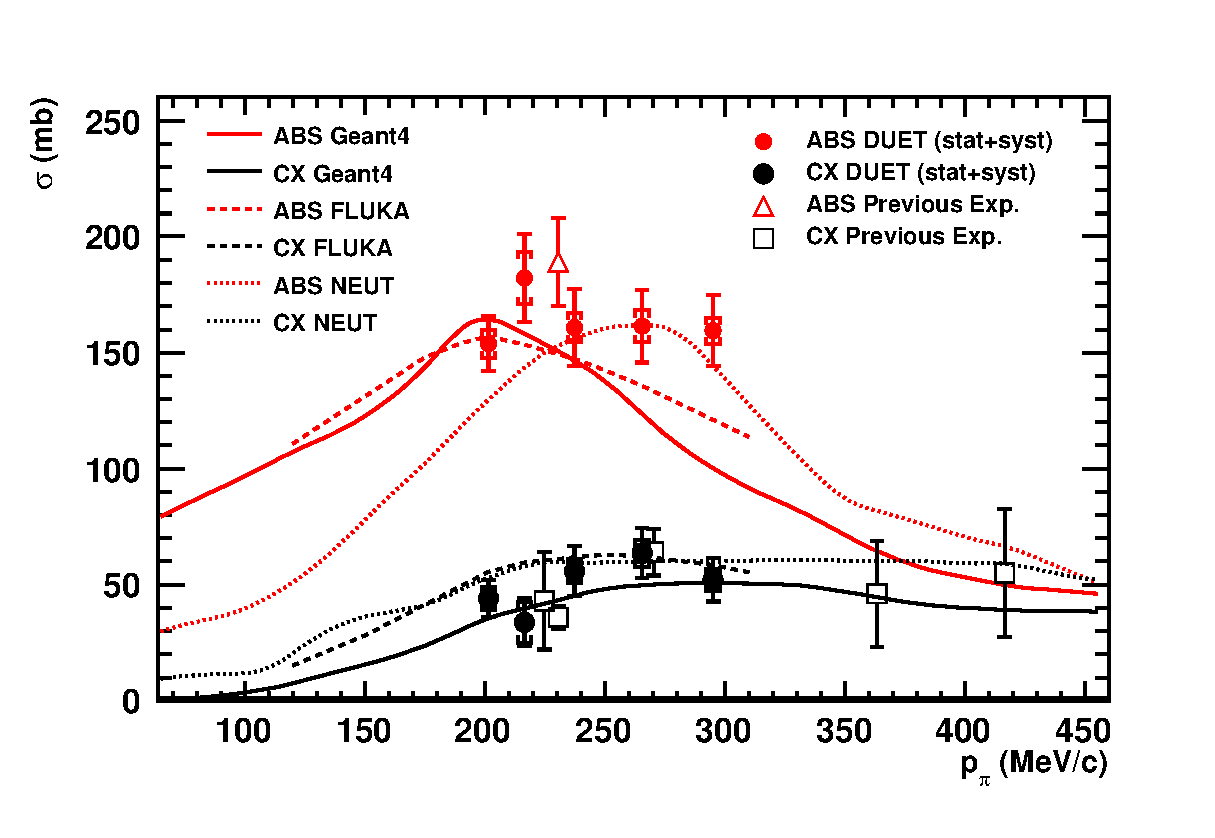
\includegraphics[width=86mm]{figures/duet_result_for_sep_paper_v2.eps}
\caption{(Color online) DUET measurements of $\sigma_{\mathrm{ABS}}$ and $\sigma_{\mathrm{CX}}$ compared with previous measurements and ABS (red) and CX (black) model predictions from \textsc{Geant4} (solid line), \textsc{Fluka} (dashed line) and \textsc{Neut} (dotted line).}
\label{fig:result}
\end{center} 
\end{figure}

In addition, we provide correlation and fractional covariance coefficients for the 5 $\sigma_{\mathrm{ABS}}$ and 5 $\sigma_{\mathrm{CX}}$ measured data points in Fig. \ref{fig:covariance}. The statistical uncertainties were included as an uncorrelated diagonal matrix. There are positive correlations within the $\sigma_{\mathrm{ABS}}$ and 5 $\sigma_{\mathrm{CX}}$ measurements, and negative correlations across them, as is expected from the subtraction method used. This is the first time that a correlation matrix is published for a pion inelastic cross section measurement. It is expected to provide additional insight to the proper modeling and tuning of hadron-nucleus inelastic interactions.

\begin{figure}[h]
\begin{center}
%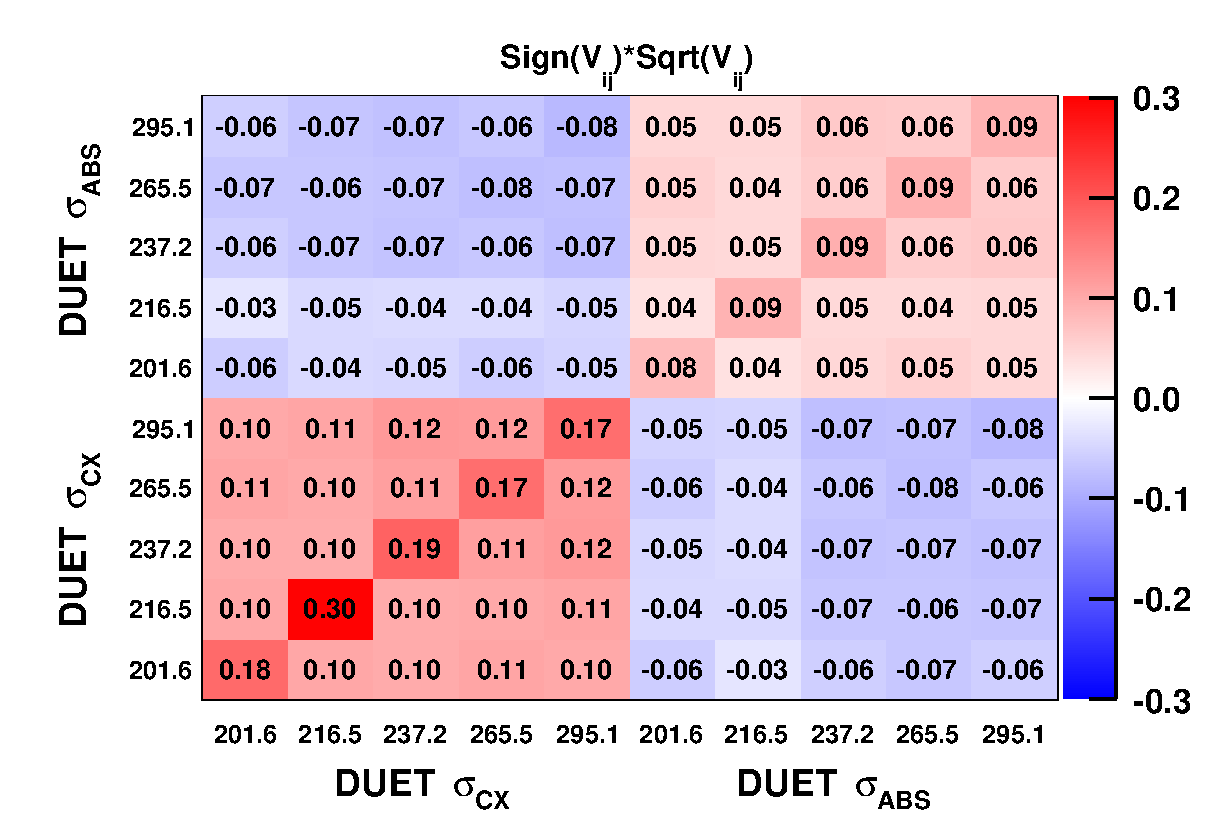
\includegraphics[width=86mm]{figures/duet_fractional_covariance_forpaper_v3.eps}
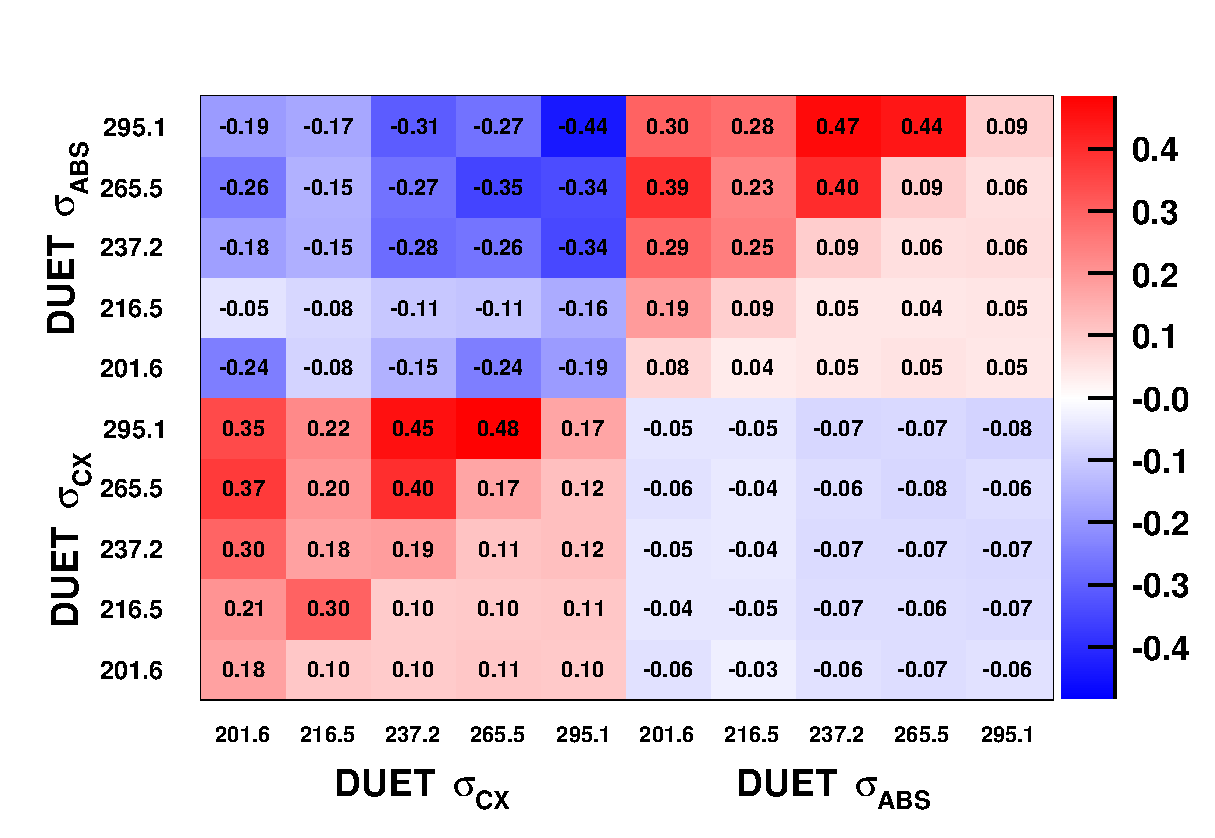
\includegraphics[width=86mm]{figures/duet_fractional_covariance_and_correlation_forpaper.eps}
\caption{(Color online) Fractional covariance and correlation for the DUET measurements of $\sigma_{\mathrm{ABS}}$ and $\sigma_{\mathrm{CX}}$. {\color{red} The upper triangle of the matrix shows the correlation coefficients, while the diagonal and lower triangle show the covariance coefficients $(\mathrm{Sign}(V_{ij})*\sqrt{V_{ij}})$.}}
\label{fig:covariance}
\end{center} 
\end{figure}

\section{Summary}
To summarize, we obtained $\sigma_{\mathrm{ABS}}$ and $\sigma_{\mathrm{CX}}$ for positive pions in carbon nuclei at five incident momenta between 201.6 MeV$/c$ to 295.1 MeV$/c$. A covariance matrix for the 10 measured data points was produced. This result will be an important input to existing models such as \textsc{Geant4} or \textsc{NEUT} to constrain sub-GeV pion interactions.
